
\subsection{Neutrino Reconstruction}
\label{neutrino}
I AM ALWAYS APPLYING CUTS SUCH THAT 1 ISOLEP FOUND AND MC MUONS
\\\\
Pair production of W bosons at $\eP\eM$ colliders is well understood in the Standard Model. These W bosons then proceed to decay and the deacy prodcts leave signals in the detector which are used to analyse the bosons themselves. In my analysis I will be focusing on the semileptonic final state of the W pair decay specifically where the lepton is a muon (Figure.~\ref{FEY:SemileptonicDecays}).
\\\\
\begin{figure}
  \centering
  \begin{tikzpicture}
  \begin{feynman}[scale=1] % using the vertex in brackets () allows fixing of vertex
    \vertex (m) at (-1, 0);
    \vertex (n) at (0.5, 0);
    \vertex (a) at (-1.5,-1);s
    \vertex (b) at ( 1.75,-1) ;
    \vertex (c) at (-1.5, 1);
    \vertex (d) at ( 1.75, 1) ;
    \vertex (u) at ( 3.5,-1.5) {$\mu^-$};
    \vertex (v) at ( 3.5,-0.5) {$\bar{\nu}_\mu$};
    \vertex (q1) at ( 3.5, 1.5) {$q$};
    \vertex (q2) at ( 3.5, 0.5) {$\bar{q'}$};
    \vertex (i1) at (-3,-1) {$e^-$};
    \vertex (i2) at (-3, 1) {$e^+$};
    \diagram* {
      (i1) -- [fermion] (m) ,
      (i2) -- [anti fermion] (m) ,
      (m) -- [photon, edge label=$Z/\gamma$] (n),
      (b) -- [photon, edge label=$W^-$, swap] (n),
      (d) -- [photon, edge label=$W^+$] (n),
      (b) -- [fermion] (u),
      (b) -- [anti fermion] (v),
      (d) -- [fermion] (q1),
      (d) -- [anti fermion] (q2),
    };
  \end{feynman}
\end{tikzpicture}

  \begin{tikzpicture}
  \begin{feynman}[scale=1] % using the vertex in brackets () allows fixing of vertex
    \vertex (n) at (0, 0.75) ;
    \vertex (m) at (0, -0.75) ;
    \vertex (a) at (-1,-1) ;
    \vertex (b) at ( 1.25,-1) ;
    \vertex (c) at (-1, 1);
    \vertex (d) at ( 1.25, 1) ;
    \vertex (u) at ( 3,-1.5) {$\mu^-$};
    \vertex (v) at ( 3,-0.5) {$\bar{\nu}_\mu$};
    \vertex (q1) at ( 3, 1.5) {$q$};
    \vertex (q2) at ( 3, 0.5) {$\bar{q'}$};
    \vertex (i1) at (-2.5,-1) {$e^-$};
    \vertex (i2) at (-2.5, 1) {$e^+$};
    \diagram* {
      (i1) -- [fermion] (m) -- [fermion, edge label=$\nu_e$] (n),
      (i2) -- [anti fermion] (n),
      (b) -- [photon, edge label=$W^-$, swap] (m),
      (d) -- [photon, edge label=$W^+$] (n),
      (b) -- [fermion] (u),
      (b) -- [anti fermion] (v),
      (d) -- [fermion] (q1),
      (d) -- [anti fermion] (q2),
    };
  \end{feynman}
\end{tikzpicture}

  \caption{Lowest order Feynman diagram of semileptonic W pair decay in the $\mu\nubar q\qbar'$ final state at $\eP\eM$ colliders. Alternately the ${W}^{+}$ could decay leptonically, which would result in a $\mu^{+}\nu q\qbar'$ final state (not drawn).}
  \label{FEY:SemileptonicDecays}
\end{figure}

In the MC simulation, there is one hard collision simulated, as well as a bunch of overlay particles, which are importent to model the spectator interstions of the other, non colliding, particles in the bunch. We need to make sure that these extra particles are not included in the reconstruction of the hard intertion. I used 'Fastjet' ***CITE*** processors to remove the overlay from the collection and to find the 2 jets corresponding to the 2 quarks in the final state. I also used the 'MyIsolatedLeptonTagger' ***CITE*** processor to extract the lepton from the recontructed particles. These three extracted particles make up the 'visible' portion of the system. The hadronically decaying W boson can be simply reconstructed by summing the 4-momenta of the 2 extracted quarks it decays into.
\\\\
The leptonically decaying W boson can similarly be reconstructed by summing the 4-momenta of the extracted lepton and the neutrino, however, the neutrino does not leave a signal in the detector. There is also some initial state radiation of photons (ISR) which are aligned enough to the beam pipe that they are lost. This results in an 'invisible' system that is not at all detected by the detector, we must therefore come up with a way to attain the 4-momenta of these invisible particles if we wish to have complete information about the W bosons.
\\\\
The chosen method for reconstruction of the invisible system arises from purely conservation laws\footnote{ a full mathematical derivation is included in the appendix for completeness (\ref{SEC:Appendix})}. We consider the reconstructed visible system as being the hadronically decaying W boson plus the isolated lepton (${p}^{\mu} = ( E,  {p}_{x}, {p}_{y}, {p}_{z})$), and the invisible system as the accompanying neutrino and an ISR photon travelling parallel to the beam. We also assume the total center of mass energy is 500 GeV and that we are in the zero momentum frame (ZMF). Conservation of momentum and energy then gives us the 4-momenta of the ISR photon and the neutrino. In the MC simulation there are actually two ISR photons emitted, this menas that when combining the two photons into one 'photon', this 'photon' may have a non zero invarient mass. The ISR photon could be going in either direction with respect to the beam axis, resulting in two soltuions.
\begin{align}
\label{EQ:full}
{E}_{\gamma}    &= \frac{{\lambda}(500 - E)  \pm {p}_{z}\sqrt{ {\lambda}^{2} - [{(500 - E)}^{2} -{p}_{z}^{2}]{m}_{\gamma}^{2}}}{{(500 - E)}^{2} -   {p}_{z}^{2}}
   \end{align}
 where $ {\lambda} = \frac{1}{2}[{(500 - E)}^2 - {p}^{2} + {m}_{\gamma}^{2} - {m}_{\nu}^{2}] $ has been defined for convenience and no absolute values have been assumed.
\\\\
 My code will then select the solution that gives a better estimate for the invarient mass of the W boson. As described in ***CITE*** this might introduce a bias and so the appropriate cut was made to mitagate this.
\\\\
 It is worth noting at this point that it is numerically possible for the particle reconstruciton to result in a visible 4-momenta with a negative $\lambda$. It can be seen in the ${m}_{\gamma} = {m}_{\nu} =0$ solution that this corresponds to the invisible part of the system having an imaginary invariant mass.
\\
 \begin{align}
 {\lambda}_{{m}_{\gamma}, {m}_{\nu} = 0} \propto {(500 - E)}^2 - {p}^{2} &= {E}_{inv}^2 - {p}_{inv}^{2} = {m}_{inv}^2
      \end{align}
\\
 This is obviously not physical and will affect the solutions attained above. For example as ${p}_{\gamma}= \pm {E}_{\gamma}$,  a negative energy will reverse the direction of the photon. This needs to be handled carefully in the code to avoid inconsistent solutions.
\\\\
 A simplified form of this equaiton with ${m}_{\gamma}= \pm {m}_{\nu} = 0$ is used in the thesis by I.M ***CITE*** that I am basing this analysis on.
 \begin{equation}
   {E}_{\gamma} = \frac{ {(500 - E)}^2 - {p}^{2}}{1000 -2 E  \mp 2{p}_{z}}
\end{equation}
\\\\
In the derivation I show how the full equation above leads to this when simplified, there is however one subtlty when this is done computationally. The $\sqrt{ {\lambda}^{2}}$ will computationally evaluate as $|{\lambda}|$, so if $\lambda$ is negative it will in effect reverse the effect of the $\pm$ in Equation.~\ref{EQ:full} and lead to the opposite solution found using the simplified form. So it is clear that these negative $\lambda$'s may cause some issues.
\\\\
 Using this method I was able to extract the 4-momentum of the leptonically decaying W boson. As a test of the performance of this code I chose to look at the reconstructed invarient mass, to see how accuratly it was reproduced. A peak at around 80 GeV was producted which is close to the currently accepted measurement of 80.3 ***CITE*** which is good, so I explored a few different variables . I found that boosting into the ZMF improved the reconstruction of the mass as is expected (Figure.~\ref{SUBFIG:Boost}). I found that including the true invarent mass of the ISR photon (collected from the simulated MC particle collection performed worse than just setting it to zero (Figure.~\ref{SUBFIG:Mass}).
\\\\
\begin{figure}
  \centering
  \begin{subfigure}[t]{0.45\textwidth}
    \centering
    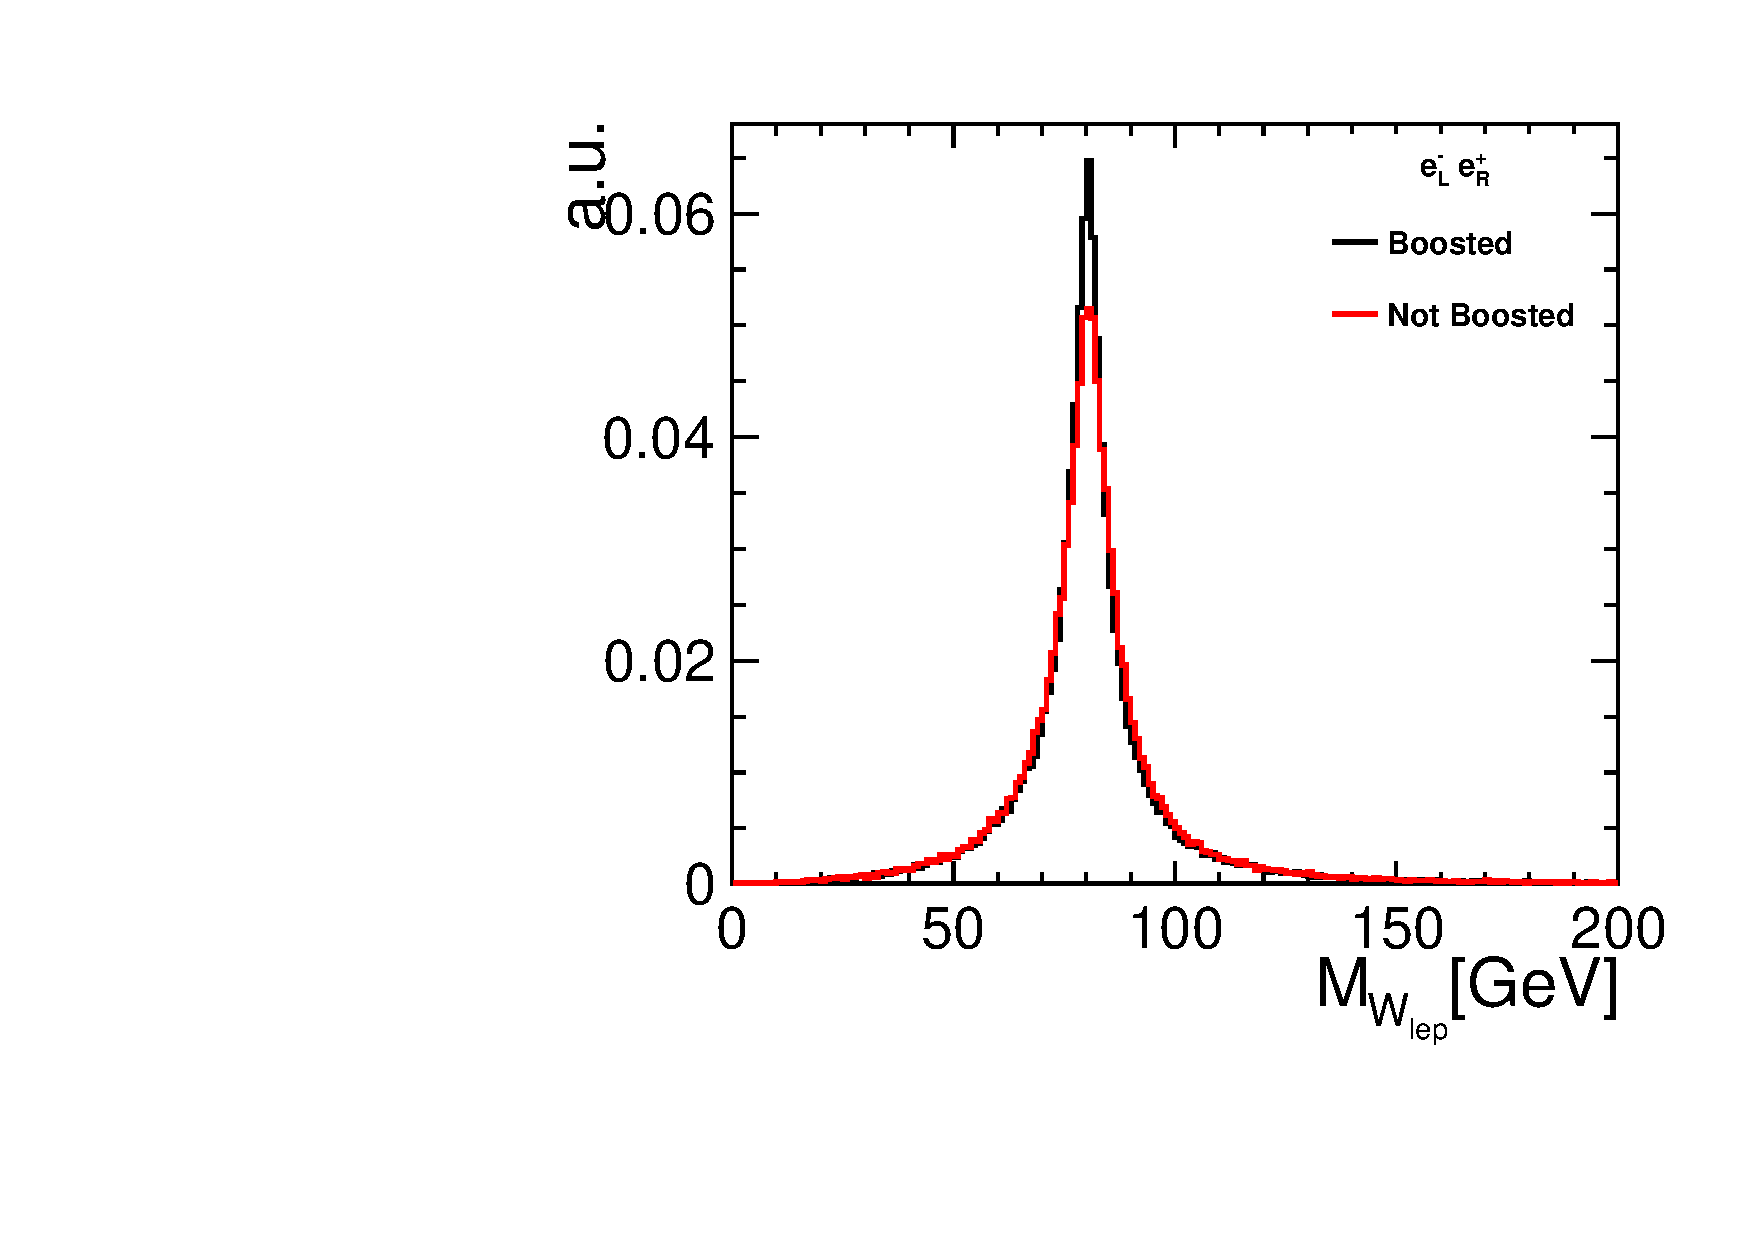
\includegraphics[width=\textwidth]{\imagepath/Boost.pdf}
    \caption{}
    \label{SUBFIG:Boost}
  \end{subfigure}
  \begin{subfigure}[t]{0.45\textwidth}
    \centering
    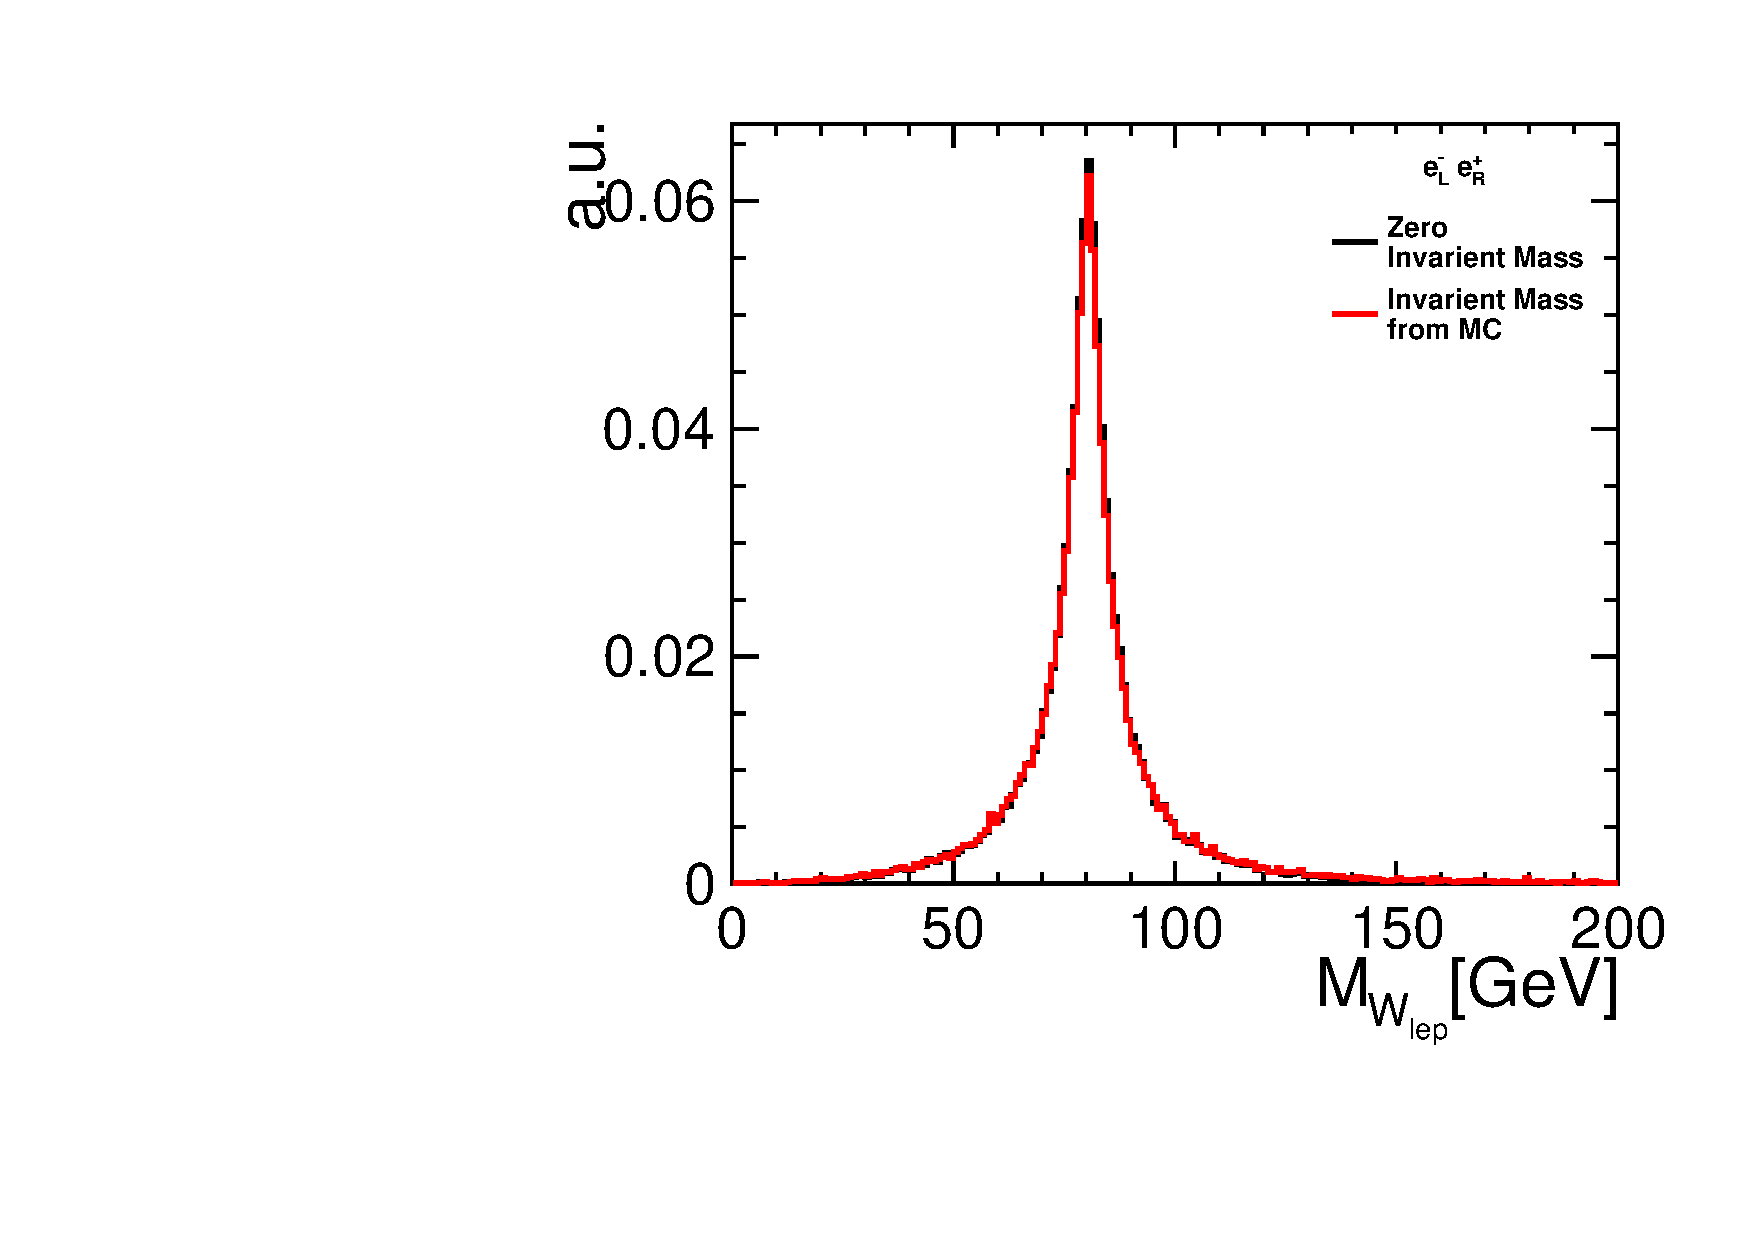
\includegraphics[width=\textwidth]{\imagepath/Mass.pdf}
    \caption{}
    \label{SUBFIG:Mass}
  \end{subfigure}
  \caption{
    Plots displaying the effect on the reconstructed invarient mass of the leptonically decaying W with different reconstruction methods.
    The simulated $\eP\eM$ collision is not head on, but with a finite momentum in the x direction, \subfigref{SUBFIG:Boost} shows the effect of boosting into the ZMF before applying the reconstruction method.
    \subfigref{SUBFIG:Mass} shows the effect of inputting a non-zero invarient ISR photon mass into the reconstruction (extracted from the MC collection).
    }
  \label{FIG:MyPlots}
\end{figure}
 I also found that cheating the overlay removal process with the 'TJJetOverlayRemoval' ***CITE*** processor peformed worse than properly using the 'Fastjet' overlay removal (Figure.~\ref{FIG:MyPlots2}). However, when we loot at the reconstruction of the hadronically decaying W boson it performs significantly better.
\\\\
\begin{figure}
    \begin{subfigure}[t]{0.45\textwidth}
      \centering
      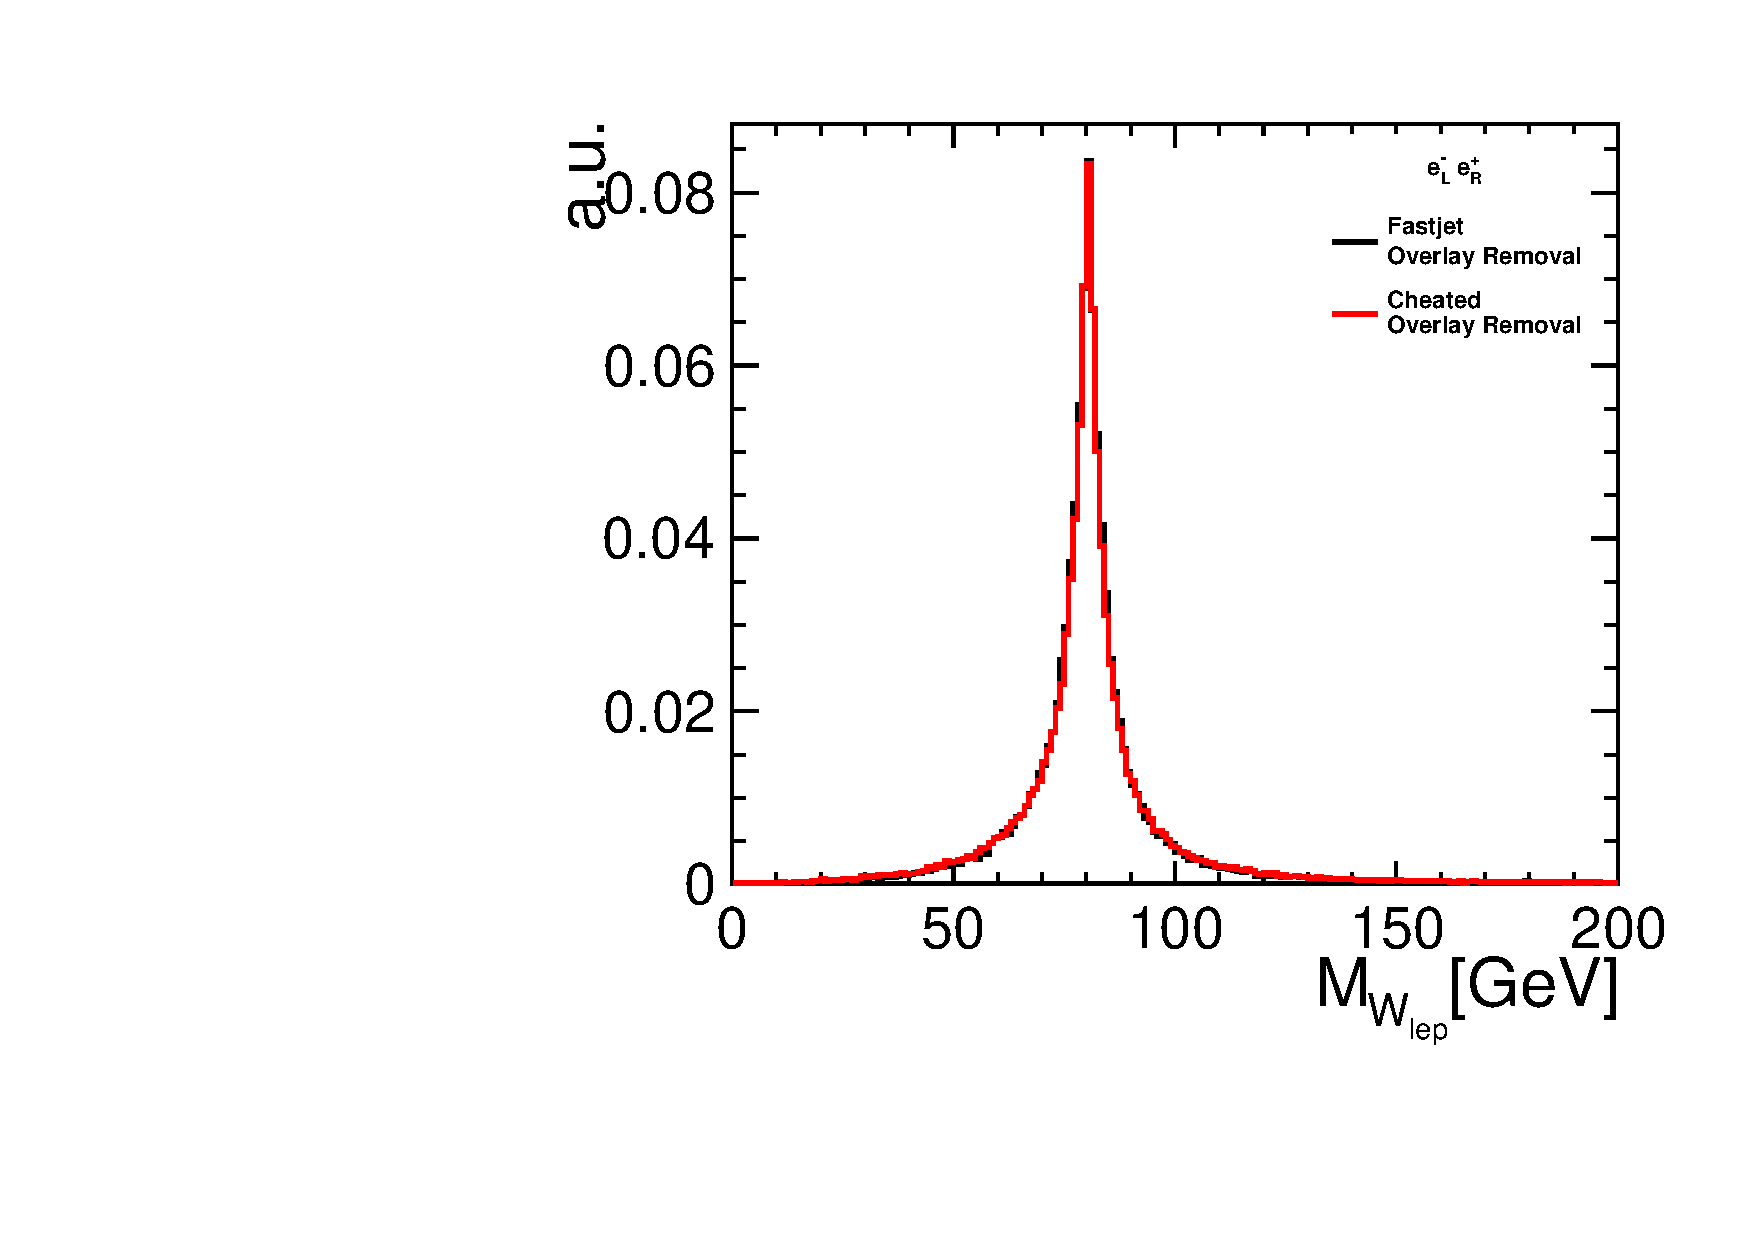
\includegraphics[width=\textwidth]{\imagepath/Lep.pdf}
      \caption{}
      \label{SUBFIG:CheatLep}
    \end{subfigure}
    \begin{subfigure}[t]{0.45\textwidth}
      \centering
      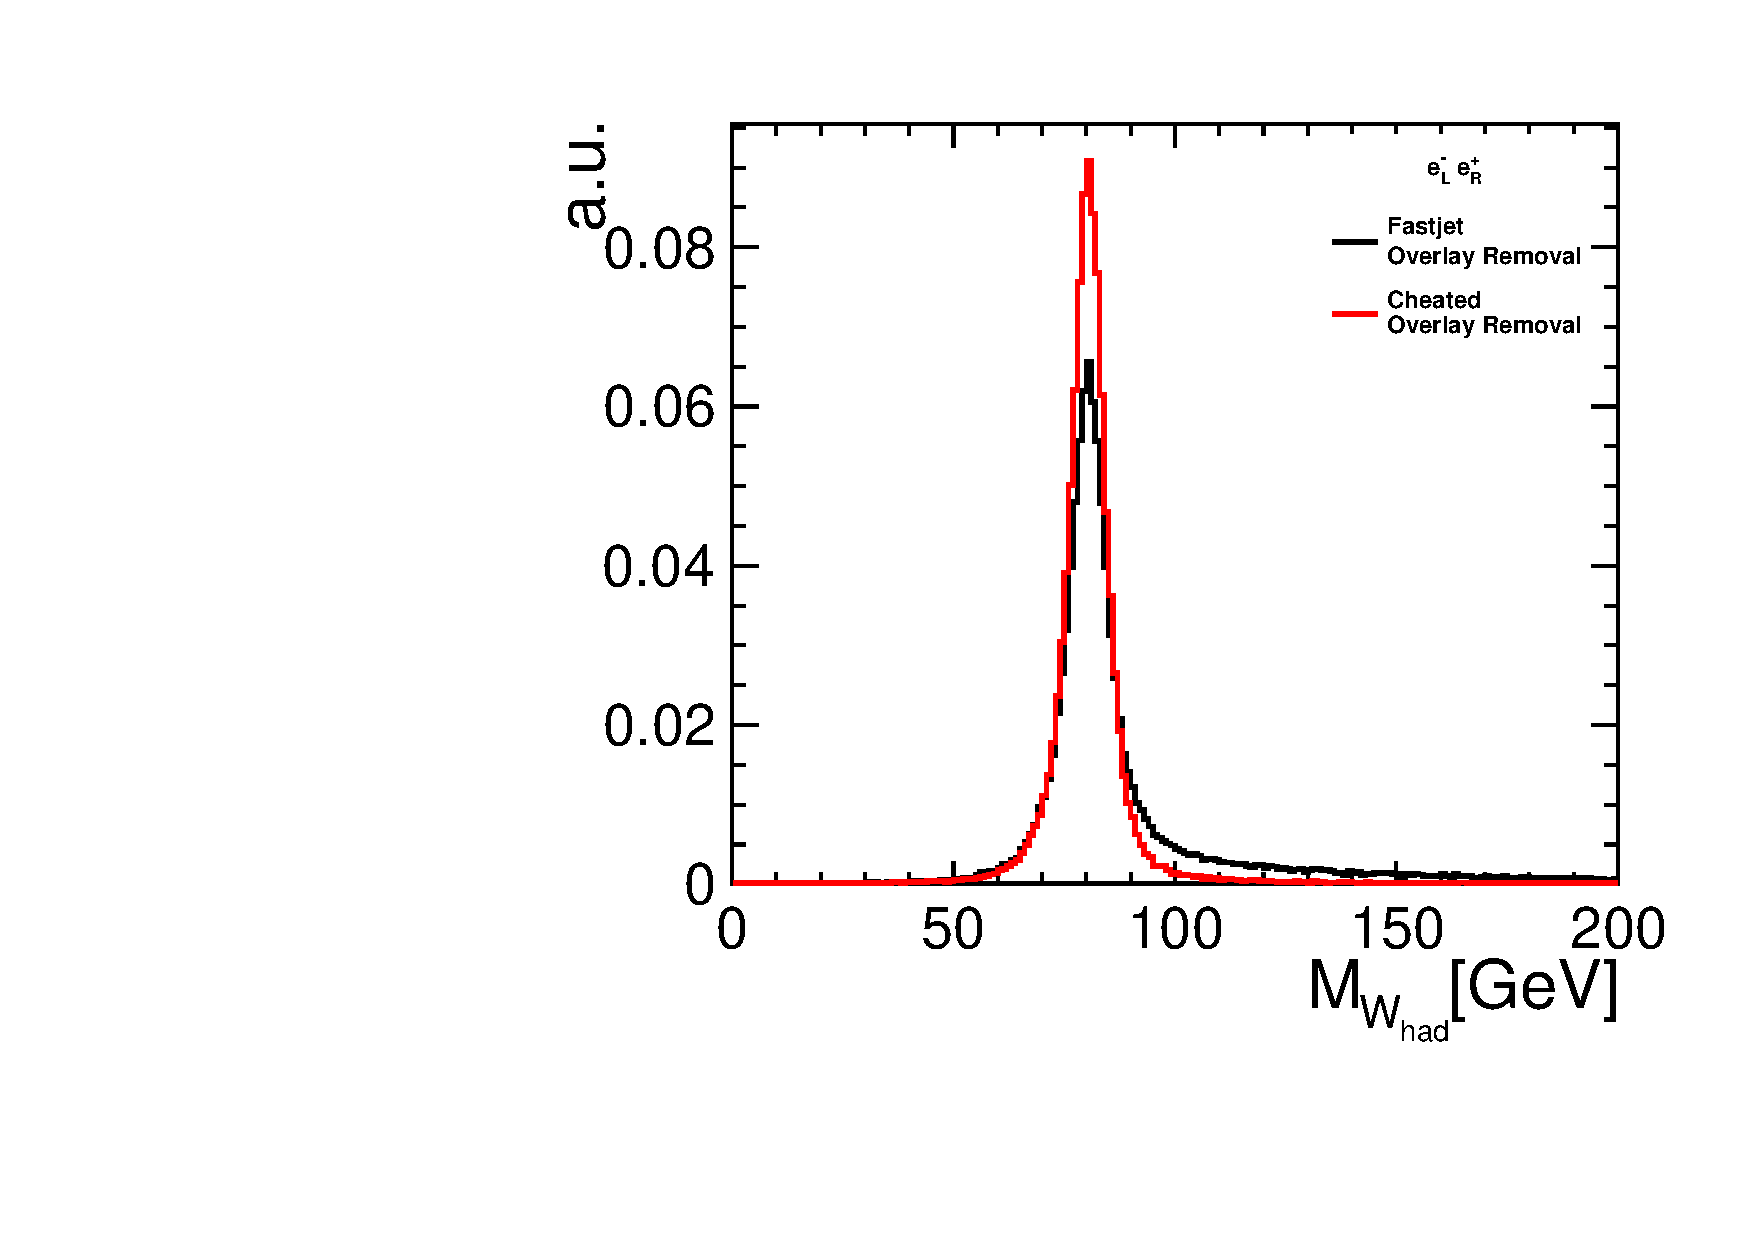
\includegraphics[width=\textwidth]{\imagepath/Jet.pdf}
      \caption{}
      \label{SUBFIG:CheatHad}
    \end{subfigure}
    \caption{
      \subfigref{SUBFIG:CheatLep} shows how cheating the overlay removal effects the reconstruction of the leptonically decaying W mass.
      \subfigref{SUBFIG:CheatHad} shows how cheating the overlay removal effects the reconstruction of the hadronically decaying W mass.
      }
    \label{FIG:MyPlots2}
\end{figure}
 Both of these results are slightly concerning as when provided with extra information, that would not be available at a real detector, the reconstruction performs worse than if this extra informaiton is withheld.
\\\\
 In my code I also gave the option for there to be no ISR photon, because there may be some computational issues ***CITE??*** with the formula at low photon energies, and calculated the kinematics as though the only invisible particle was the neutrino. I then observed the effect this had on the boson mass distributions (Figure.~\ref{FIG:STUFF}). It appears that including this options significantly improves the estimations, however I had to check that this isn't just a statistical bais of adding a third possible option to get closer to the true mass. So in Figure.~\ref{FIG:Photon} I plotted the reconstructed photon energy that would have been chosen were there no ${E}_{ISR}=0$ option agains the true MC photon energy, for the events where the full simulation chose the ${E}_{ISR}=0$ option. We see no real correlation forming which is good becuase it means the ${E}_{ISR}=0$ option isnt performing worse, and we see that most of the times when this performed better was at particulatrly low ${E}_{MC}$ values where the formual struggled to get an accurate reconstruction of the photon energy.
 \\\\
 \begin{figure}
   \centering
   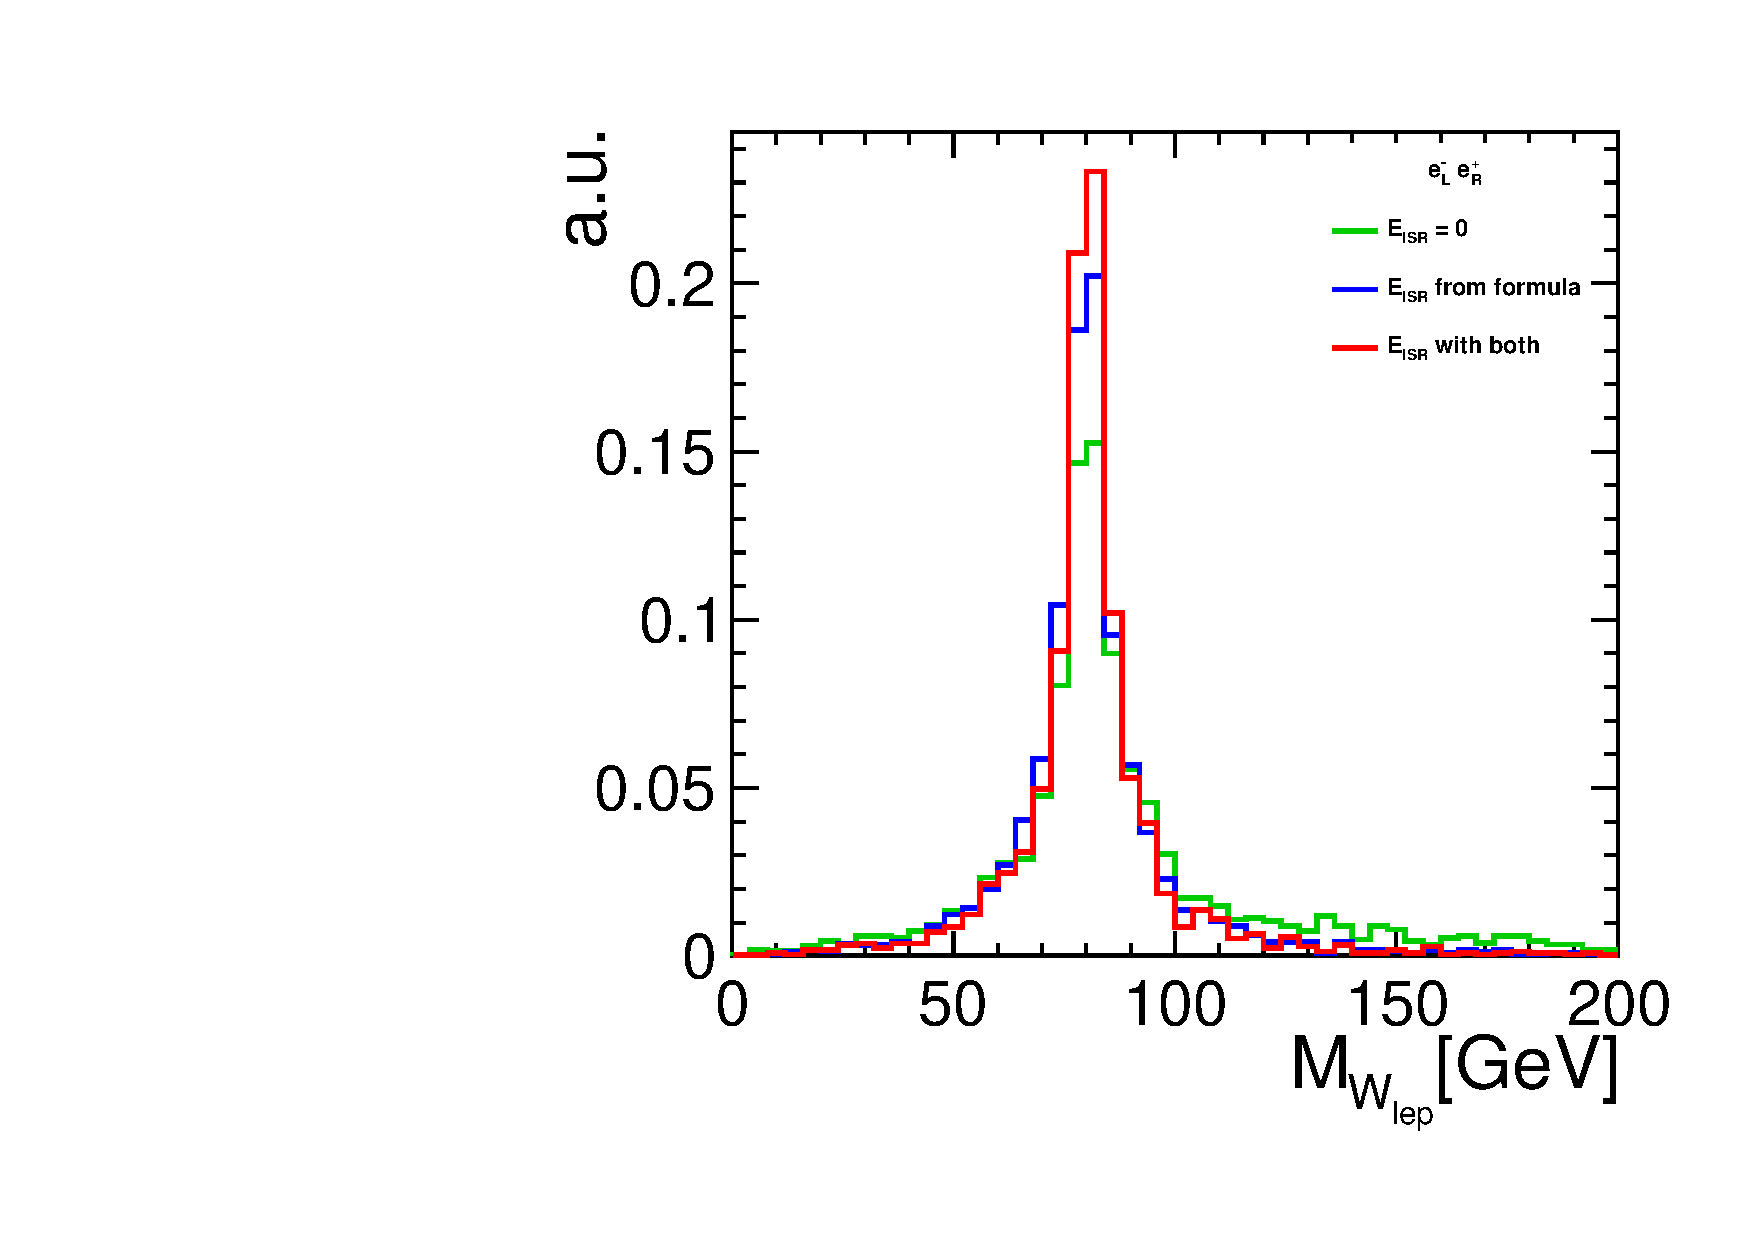
\includegraphics[width=\textwidth]{\imagepath/Mass3.pdf}
   \caption{
   Histogram showing how well the 3 different ${E}_{\gamma}$ claculation methods reconstruct the leptonically decaying W mass.
   }
   \label{FIG:STUFF}
 \end{figure}
\begin{figure}
  \centering
  \begin{subfigure}[t]{0.45\textwidth}
    \centering
    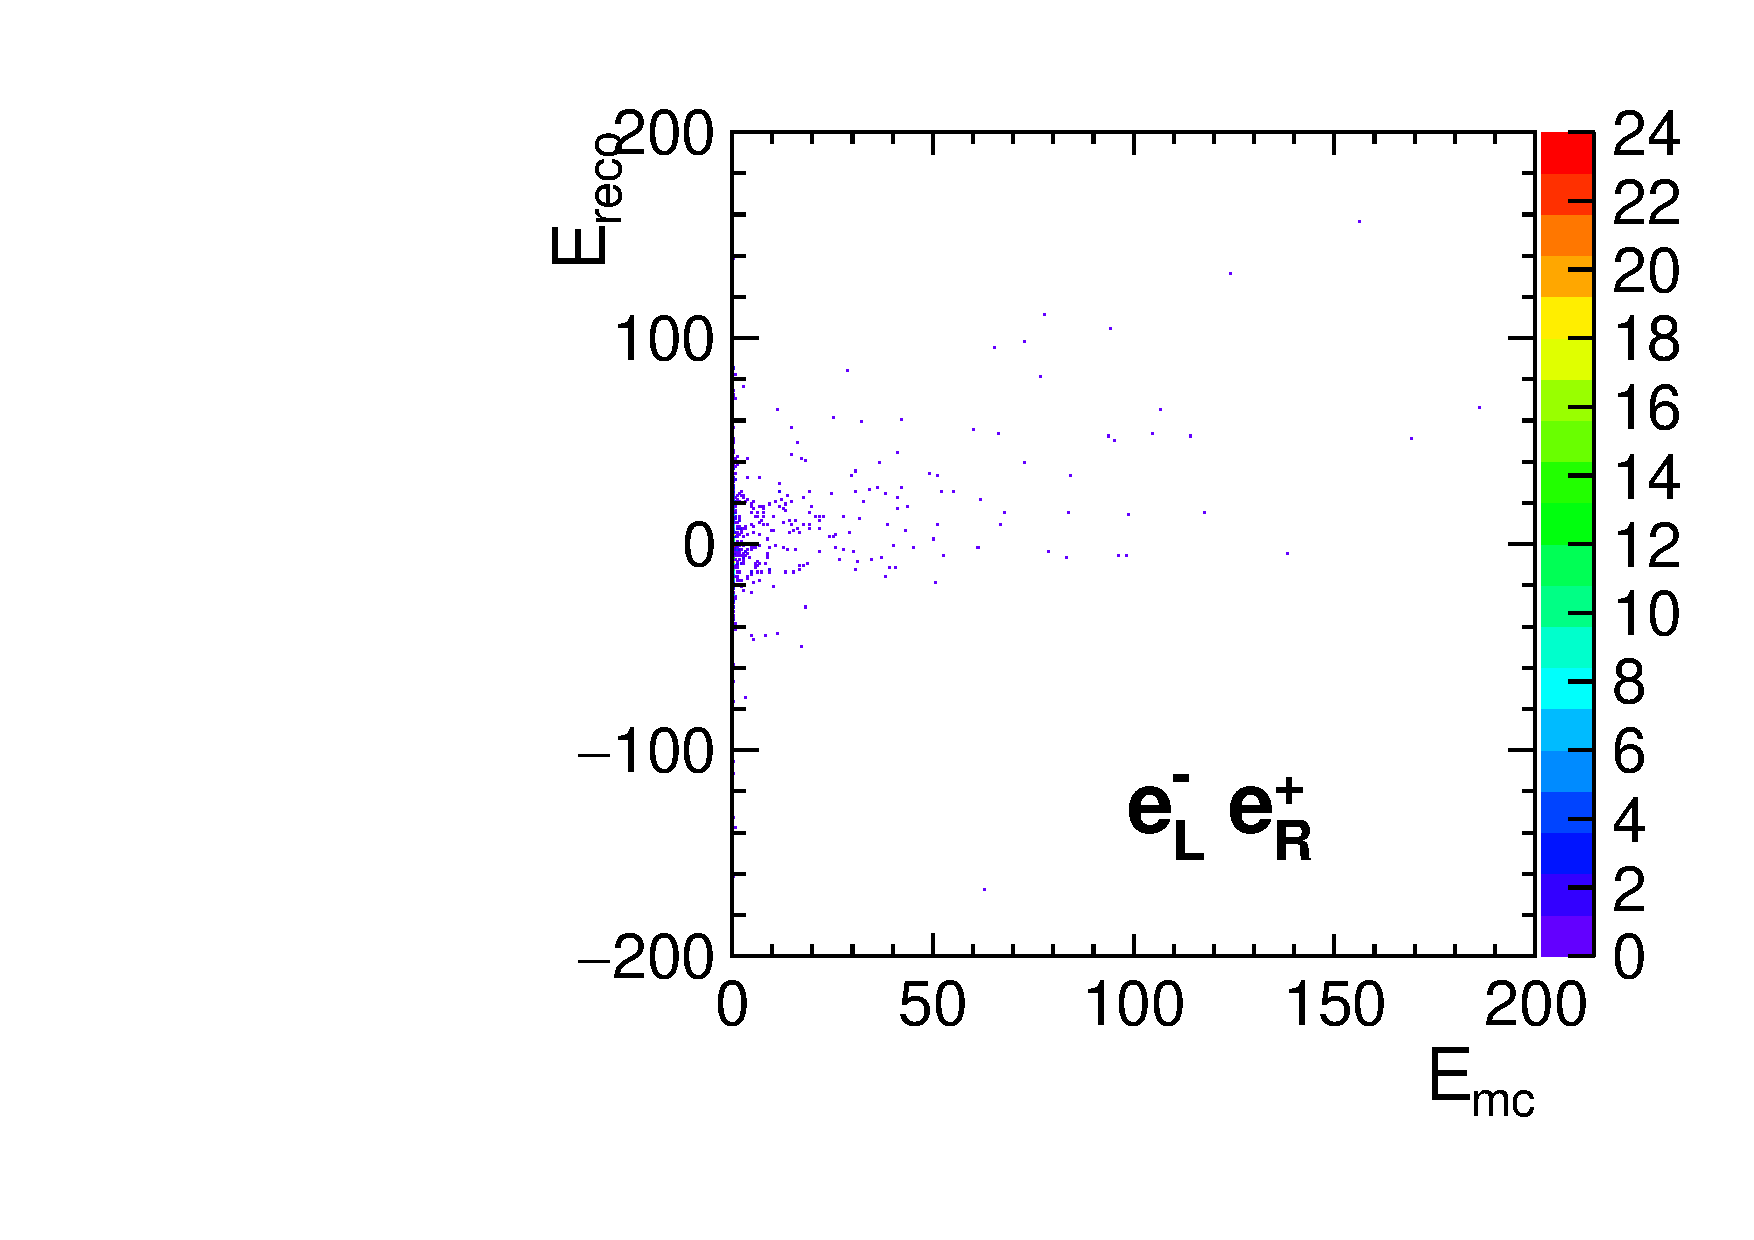
\includegraphics[width=\textwidth]{\imagepath/Photon.pdf}
    \caption{}
    \label{SUBFIG:Photon_full}
  \end{subfigure}
  \begin{subfigure}[t]{0.45\textwidth}
    \centering
    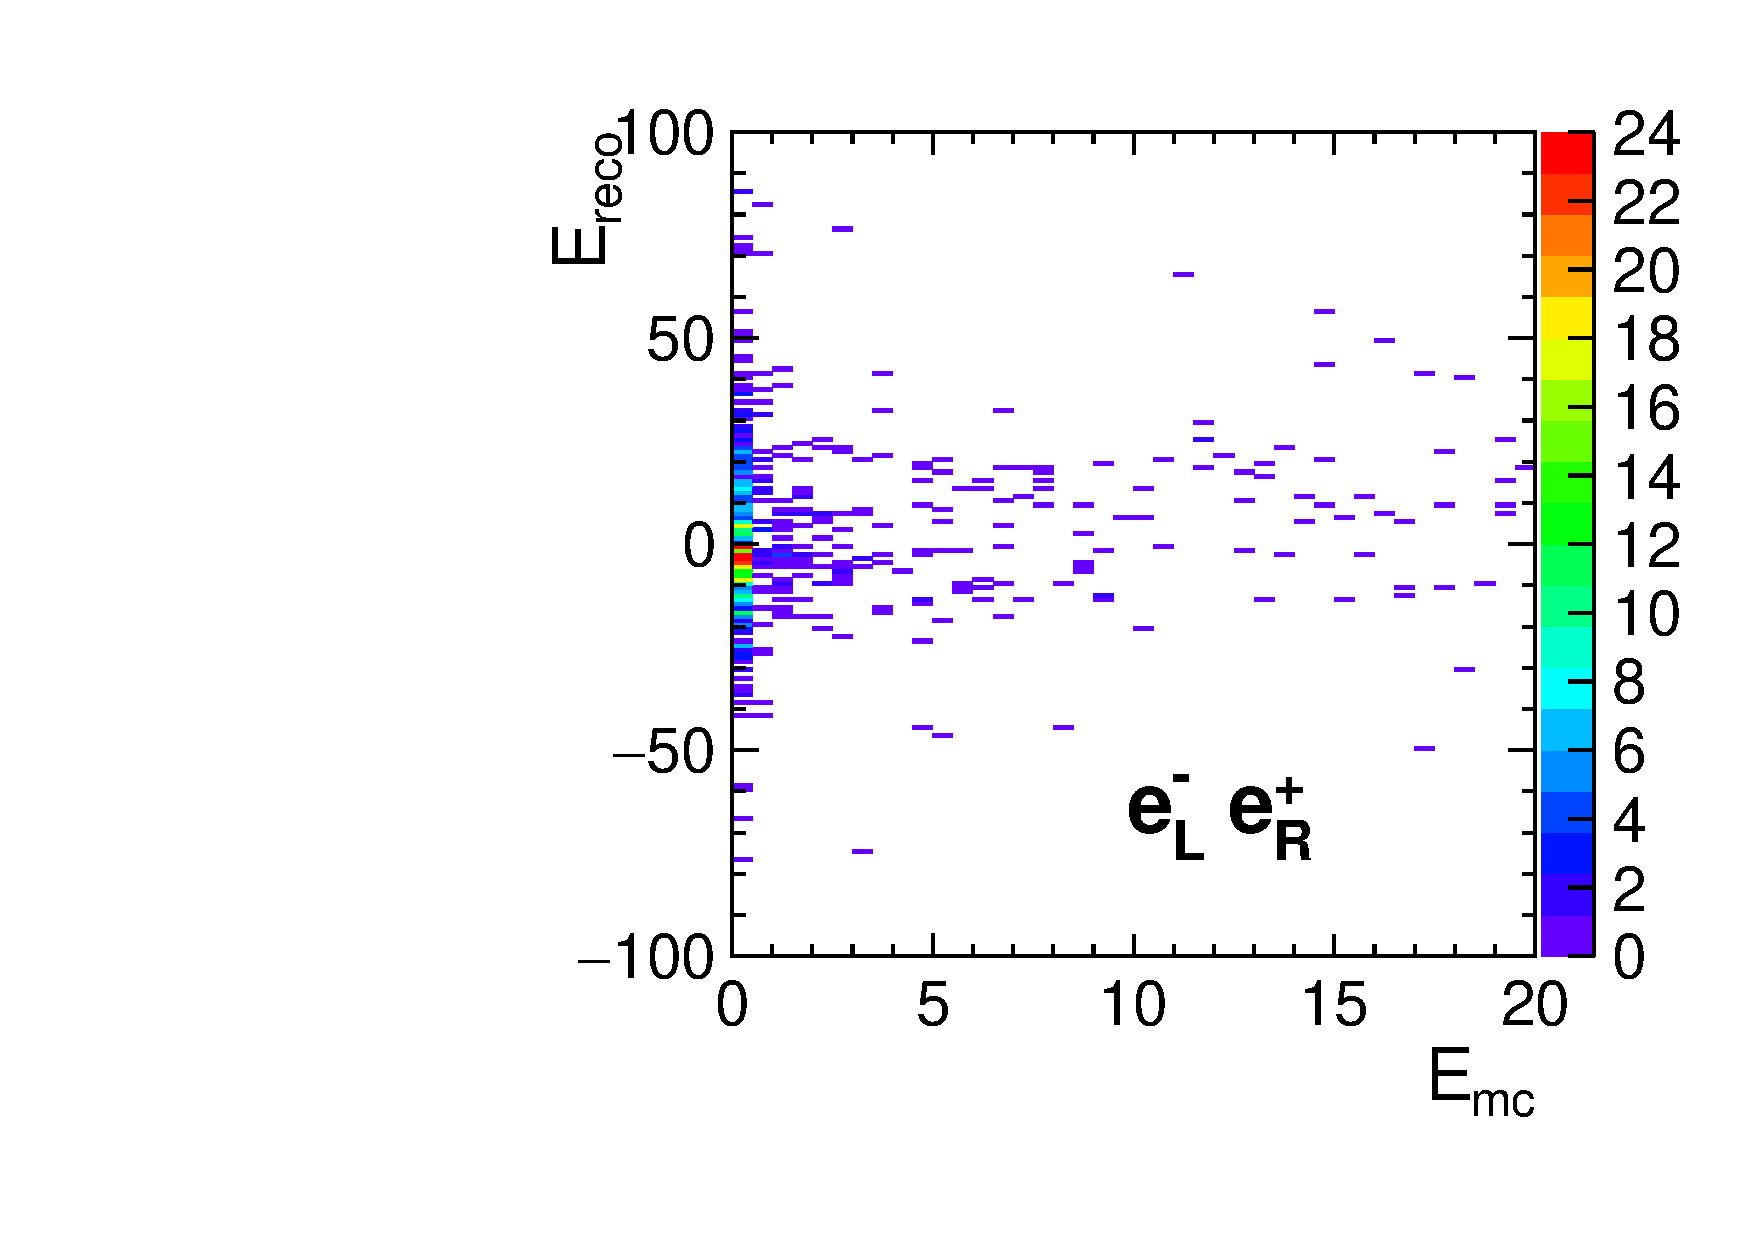
\includegraphics[width=\textwidth]{\imagepath/Photon_zoom.pdf}
    \caption{}
    \label{SUBFIG:Photon_zoom}
  \end{subfigure}
  \caption{
    This figure shows the distribution of photon energies from the formula that would have been chosen were there no ${E}_{ISR}=0$ option agains the true MC photon energy, for the events where the full simulation chose the ${E}_{ISR}=0$ option. \subfigref{SUBFIG:Photon_zoom} is the same plot as \subfigref{SUBFIG:Photon_full} with a restricted axis range for clarity.
  }
  \label{FIG:Photon}
\end{figure}

My only current explation for this is that the formula is rather un-sensitive to this change, and so the slight decrease in performance of the ${m}_{W}^{lep}$ estimation is just a statistical fluctuation from the formula.
\\\\
I then apply all of the cuts outlined in I.M. ***CITE*** thesis and see how this effects the selection efficiency. From here on I will be using the method above choosing the best of all 3 possible ${E}_{\gamma}$ solutions with ${m}_{\gamma}= {m}_{\nu} = 0$. Applying the cuts outlined in Table.~\ref{TAB:SelectionEfficiencies}, I arrive at an efficiency flow diagram (Figure.~\ref{FIG:Flow}).
\\\\
  \begin{table}[!]
    \centering
    \caption{
      Selection efficiency of sequantially applied cuts. Where the post ISR correction ${m}_{W}^{lep}$ was calculated using all 3 possible ${E}_{\gamma}$ solutions. (*) Means my and Ivan's cuts differ slightly
    }
    \label{TAB:SelectionEfficiencies}
        \resizebox{0.8\textwidth}{!}{%
        \begin{tabular}{|l|l|l|l|l|} \hline
          Order & Cut description & \multicolumn{3}{c|}{Efficiency [\%]} \\ \cline{3-5}
          & & \multicolumn{2}{c|}{My Results} & Ivan's Results \\  \cline{3-4}
          & & n = 2129 & n = 99419 & n = 107233 \\ \hline \hline
          0 & muon signal & 100.00 & 100.00 & 100.00 \\ \hline
          1 & track multiplicity\tablefootnote{track mulitplicity was taken as the number of reconstructed charged particles.} ${n}_{tracks} \ge 10$ & 97.13 & 97.01 & 99.996 \\ \hline
          2 & center of mass energy $\sqrt{s} > 100$ GeV & 92.29 & 91.69 & 97.96 \\ \hline
          3 & total transverse momentum ${P}_{T} > 5$ GeV & 91.16 & 90.47 & 96.69 \\ \hline
          4 & total energy ${E}_{SUM} < 500$ GeV & 89.66 & 89.28 & 95.36 \\ \hline
          5 & $\ln{({y}_{+})} \in [-12, -3]$ (*) & 88.69 & 88.08 & 95.01 \\ \hline
          6 & 1 lepton found (*) & 80.65 & 80.77 & 78.75 \\ \hline
          7 & pre ISR correction ${m}_{W}^{lep} \in [20, 250]$ GeV &  78.23 & 77.94 & 76.61 \\ \hline
          8 & tau discrimination\tablefootnote{${\tau}_{discr}$ defined by ${\tau}_{discr} = {(\frac{2{E}_{lep}}{\sqrt{s}})}^{2} + {(\frac{{m}_{W}^{lep}}{{m}_{W}^{true}})}^{2}$} &  76.05 & 75.60 &  74.07 \\ \hline
          9 & charged lepton (*) & 76.05 & 75.60 & 73.51 \\ \hline
          10 & isolation variable\tablefootnote{$\Delta{\Omega}_{iso}$ defined as,
          \begin{align}
              ({\phi}_{lep} - {\phi}_{had}) < \pi \to \Delta{\Omega}_{iso} &= \sqrt{{({\theta}_{lep} - {\theta}_{had})}^{2}+{({\phi}_{lep} - {\phi}_{had})}^{2}} \\
              ({\phi}_{lep} - {\phi}_{had}) \ge \pi \to \Delta{\Omega}_{iso} &= \sqrt{{({\theta}_{lep} - {\theta}_{had})}^{2} + {(2\pi - |{\phi}_{lep} - {\phi}_{had} |)}^{2}} \, .
          \end{align}} ${\Delta\Omega}_{iso} > 0.5$ & 76.01 & 75.58 & 73.42 \\ \hline
          11 & post ISR correction ${m}_{W}^{lep} \in [40, 120]$ GeV & 72.90 & 72.77 & 70.13 \\ \hline
          12 & post ISR correction ${m}_{W}^{had} \in [40, 120]$ GeV & 63.21 & 62.92 & 66.93 \\ \hline
          13 & $\cos{{\theta}_{W}} > -0.95$ & 63.02 & 62.65 & 66.78 \\ \hline
        \end{tabular}
        }
    \end{table}

\begin{figure}
    \centering
    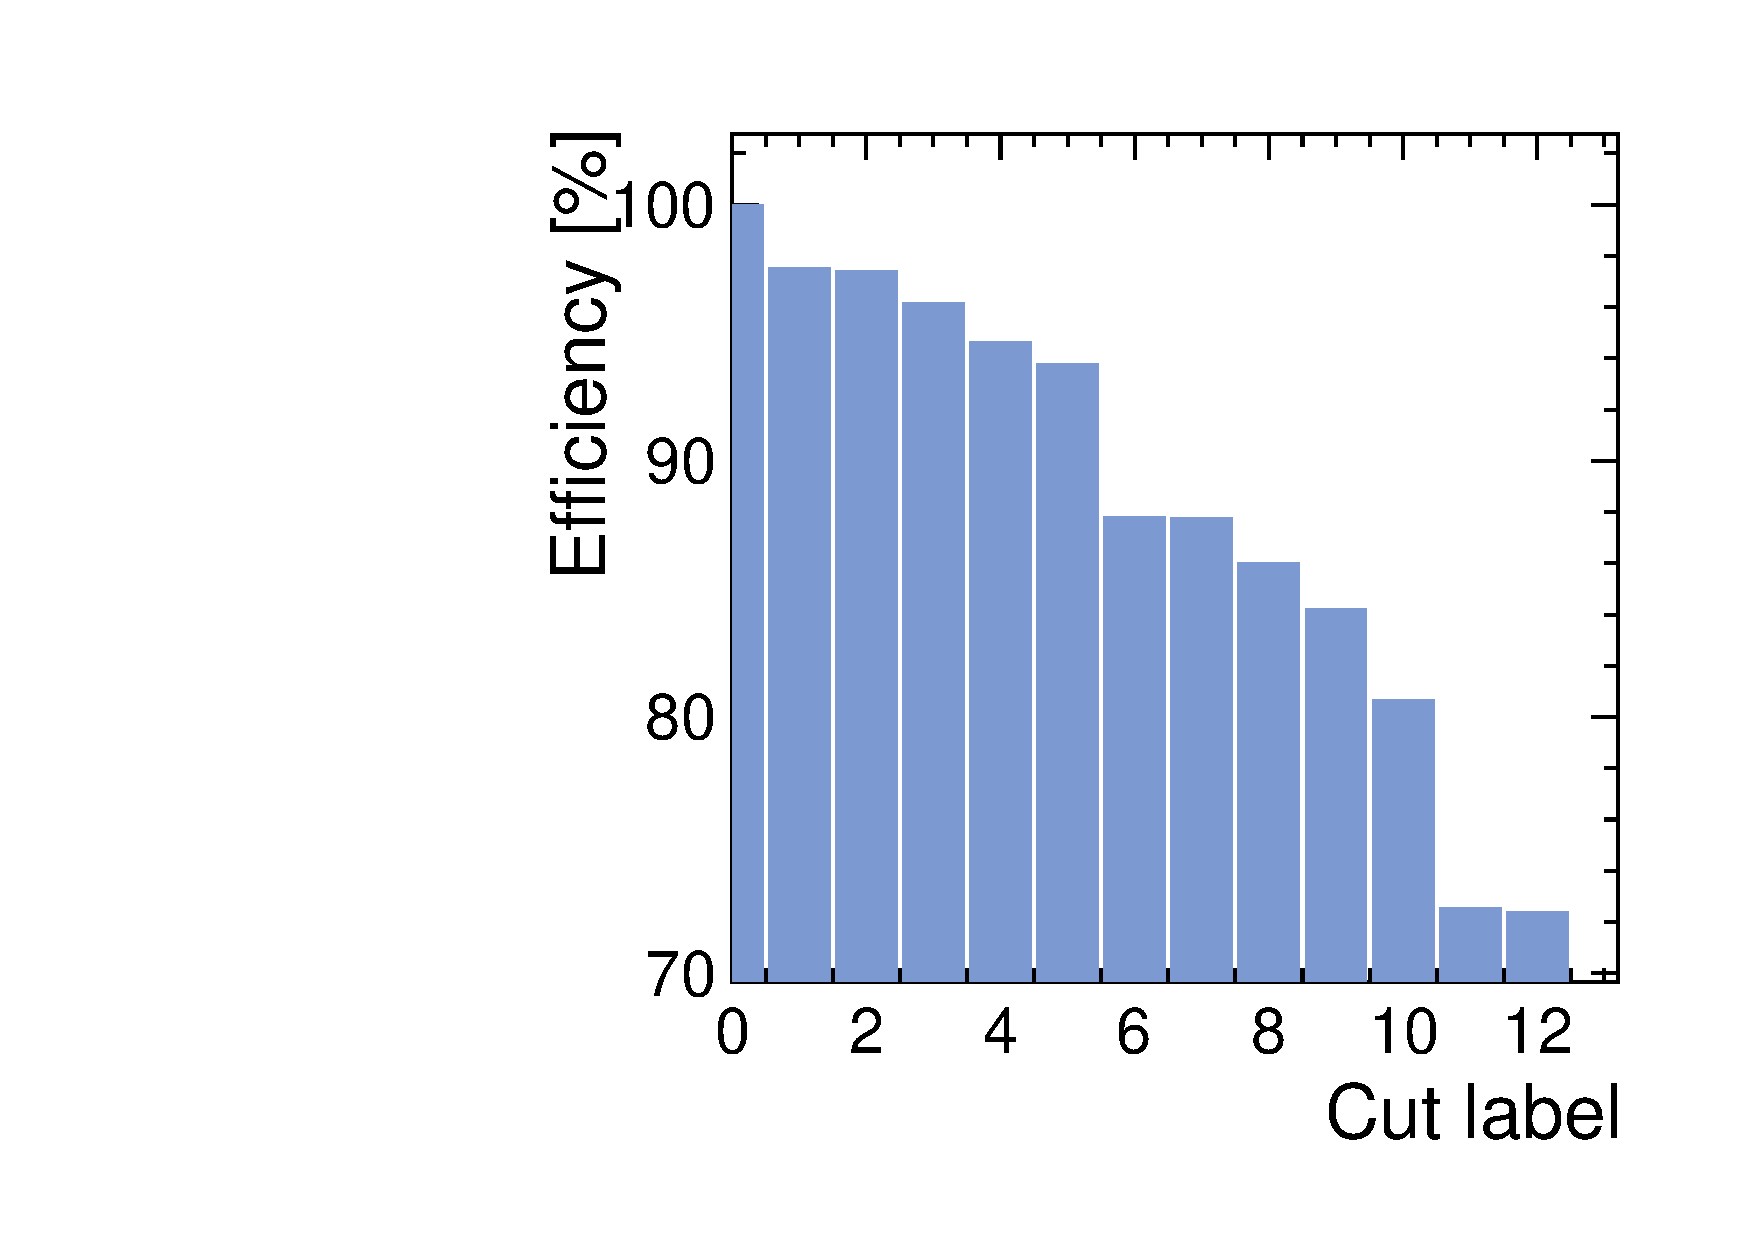
\includegraphics[width=\textwidth]{\imagepath/HistFlow.pdf}
    \caption{
    Histogram showing the cut efficiency, with the cut labels defined in Table.~\ref{TAB:SelectionEfficiencies}
    }
    \label{FIG:Flow}
\end{figure}

\subsection{Angle extractions}
\label{angles}
The next part of my project involved extracting a few angles from the hard reaction from the MC Collection. I picked out the semileptonic final state particles from the collection, and reconstructed the leptonic and hadronic jets by basic addition of the 4-momenta. It was then a simple matter of extracting the appropriate angles from the 4 momenta as described in Robert Karls thesis ***CITE*** (Figure.~\ref{FIG:MyPlots2}) from the MC collection.
\\\\
The first angle $\theta_{W^{-}}$ if defined as the angle between the negiativly charged W boson ($W^{-}$) and the beam pipe in the electron direction of travel (the z axis in the MC simuation). I extracted this in the center of mass frame of the $\eP\eM$, which required a boost of $(500\sin{(\frac{0.014}{2})}, 0, 0)$ GeV due to their non zero incidence angle. The rest of the coordinates were simply the polar coordinates of the muon, agian with z aligned to the beam pipe, in the center of mass frame of the leptonically decaying W boson (${\theta}_{l}^{*}$ and ${\phi}_{l}^{*}$) .

\begin{figure}
    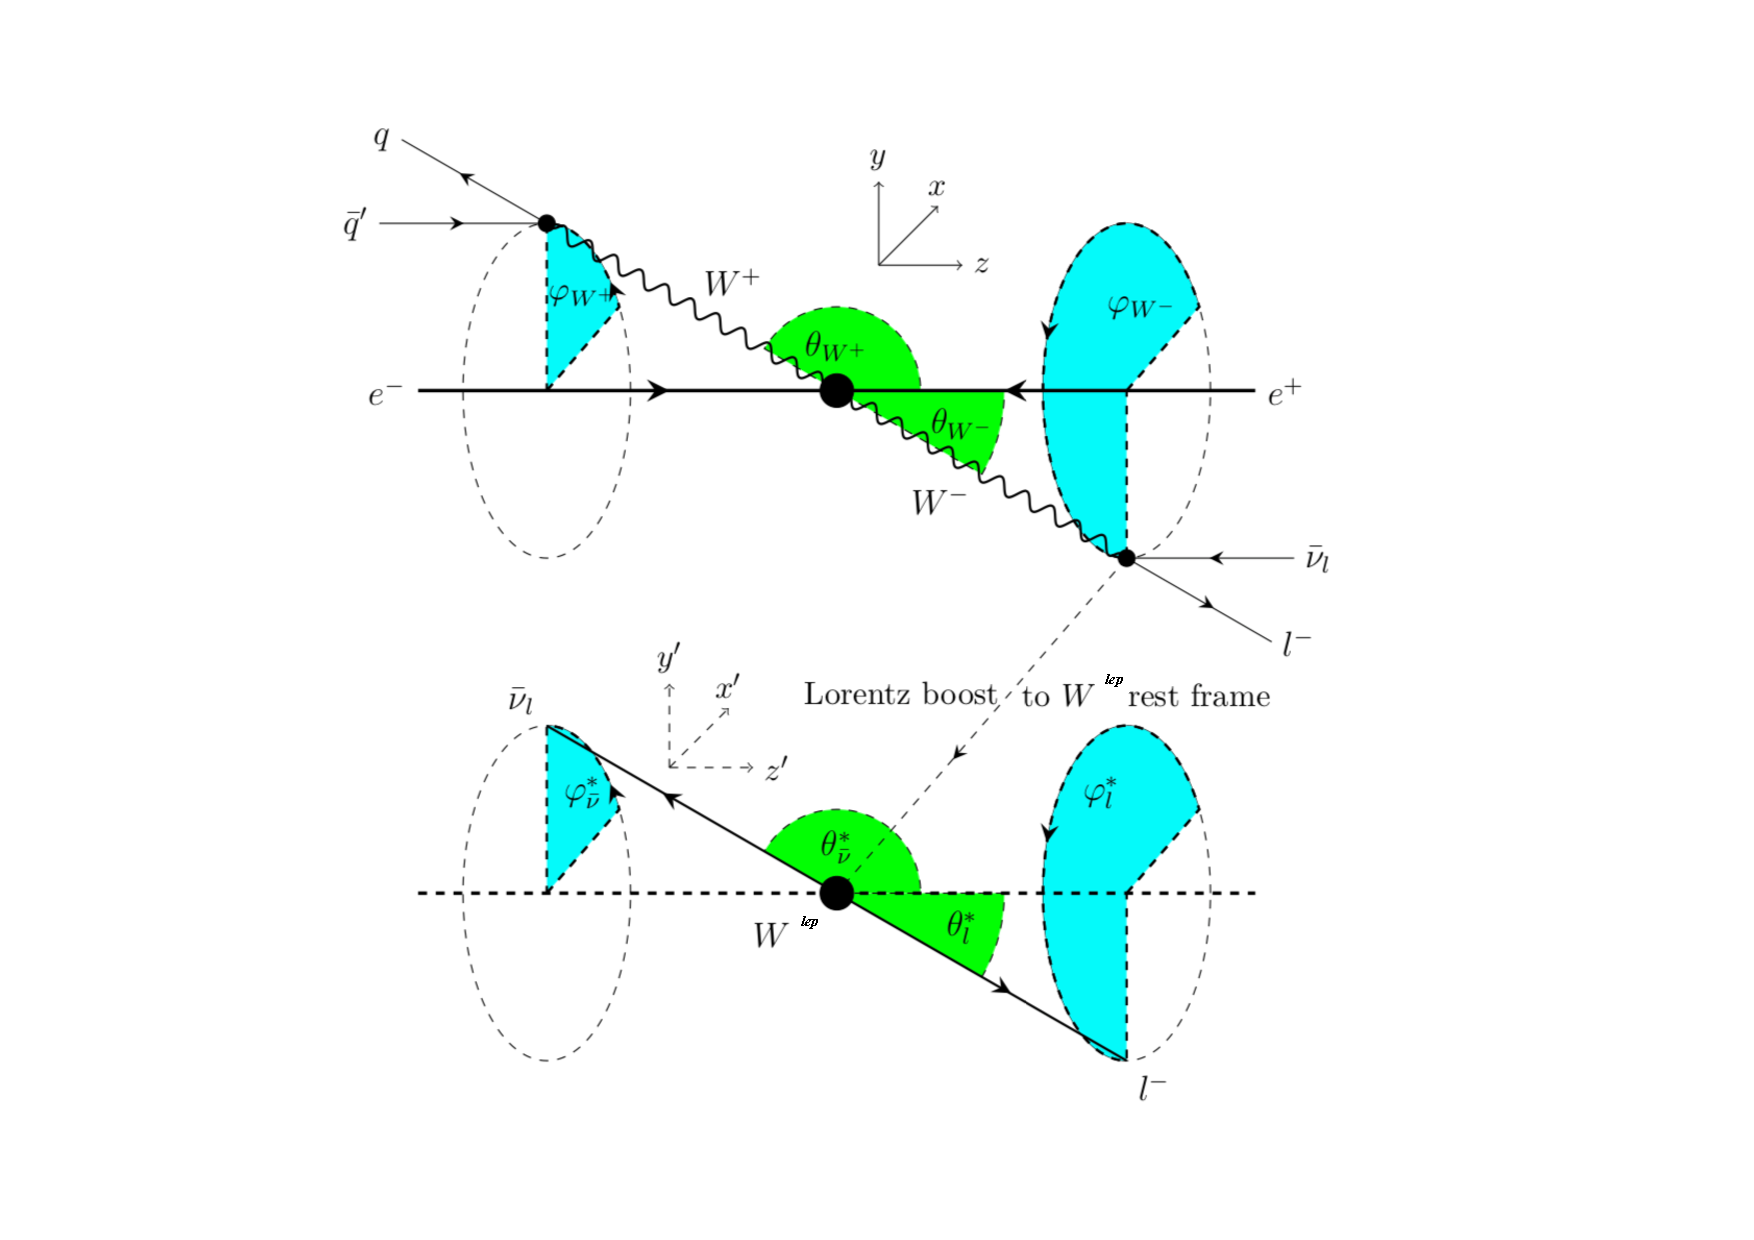
\includegraphics[width=\textwidth]{\imagepath/AngleDiag.pdf}
    \caption{
    Angle definition for the 4-fermion final state from ${W}^{-}$ pair production in the semileptonic channel in which the W− decays leptonically. In the top part, the production angles ${\theta}_{{W}^{-}}$ and ${\theta}_{{W}^{+}}$ are defined by the axis of the initial colliding particles and the direction for the respective boson. The azimuthal angles ${\phi}_{{W}^{-}}$ and ${\phi}_{{W}^{+}}$ describe the rotation around the axis of the initial colliding particles.\\
    The bottom picture shows the angular definition of the decay products of the ${W}^{lep}$ boson in its rest frame. It shows the polar angles ${\theta}_{l}^{*}$ and ${\theta}_{\nubar}^{*}$ and the azimuth angles ${\phi}_{l}^{*}$ and ${\phi}_{\nubar}^{*}$ of the corresponding leptons. The ∗ denotes quantities in the rest frame of the ${W}^{lep}$ boson. (Edited from Robert Karl ***CITE***)
      }
    \label{FIG:MyPlots3}
\end{figure}
